\acresetall
\chapter{Other Applications}
\label{ch:other}

\section{Chronic remapping}\label{sec:applications:chronic}
\todo[inline, color=yellow]{Include chronic remapping results?}

\section[Gating of hippocampal activity, plasticity, and memory by entorhinal cortex long-range inhibition]{Gating of hippocampal activity, plasticity, and memory by entorhinal cortex long-range inhibition\footnote{This work has been previously published \citep{Basu2016} and is joint work with the coauthors.}}

\begin{quote}
The cortico-hippocampal circuit is critical for storage of associational memories. Most studies have focused on the role in memory storage of the excitatory projections from entorhinal cortex to hippocampus. However, entorhinal cortex also sends inhibitory projections, whose role in memory storage and cortico-hippocampal activity remains largely unexplored. We found that these long-range inhibitory projections enhance the specificity of contextual and object memory encoding. At the circuit level, these g-aminobutyric acid (GABA)–releasing projections target hippocampal inhibitory neurons and thus act as a disinhibitory gate that transiently promotes the excitation of hippocampal CA1 pyramidal neurons by suppressing feedforward inhibition. This enhances the ability of CA1 pyramidal neurons to fire synaptically evoked dendritic spikes and to generate a temporally precise form of heterosynaptic plasticity. Long-range inhibition from entorhinal cortex may thus increase the precision of hippocampal-based long-term memory associations by assessing the salience of mnemonic information to the immediate sensory input.
\attrib{\citealt{Basu2016}}
\end{quote}

This project was primarily the work of the first author, Jayeeta Basu, who performed the slice physiological recordings characterizing this long-range inhibitory projection (LRIP) from lateral entorhinal cortex (LEC) to the \emph{stratum lacunosum moleculare} of hippocampal area CA1, which gated a a specific form of input timing-dependent plasticity between CA3 Schaffer collaterals and CA1 pyramidal cells. In addition, Dr. Basu showed that interrupting this projection \emph{in vivo} affected both context and object recognition memory. As further evidence for the \emph{in vivo} role of these LRIPs from LEC to CA1, I imaged these fibers in CA1 while mice were running and exposed to various sensory stimuli.

We found that LEC inhibitory axons in CA1 showed robust responses to aversive (air puff), appetitive (water), and contextual (tone and light) stimuli. (\autoref{fig:applications:LRIP:imaging}).
In addition, these responses were coherent across buttons on a single axons and individual boutons responded to more than 2 stimuli at a higher rate than chance, together suggesting that there is a subpopulation of LEC inhibitory projecting cells which preferentially encode contexts as a whole (\autoref{fig:applications:LRIP:boutons}).

\begin{figure}
	\centering
	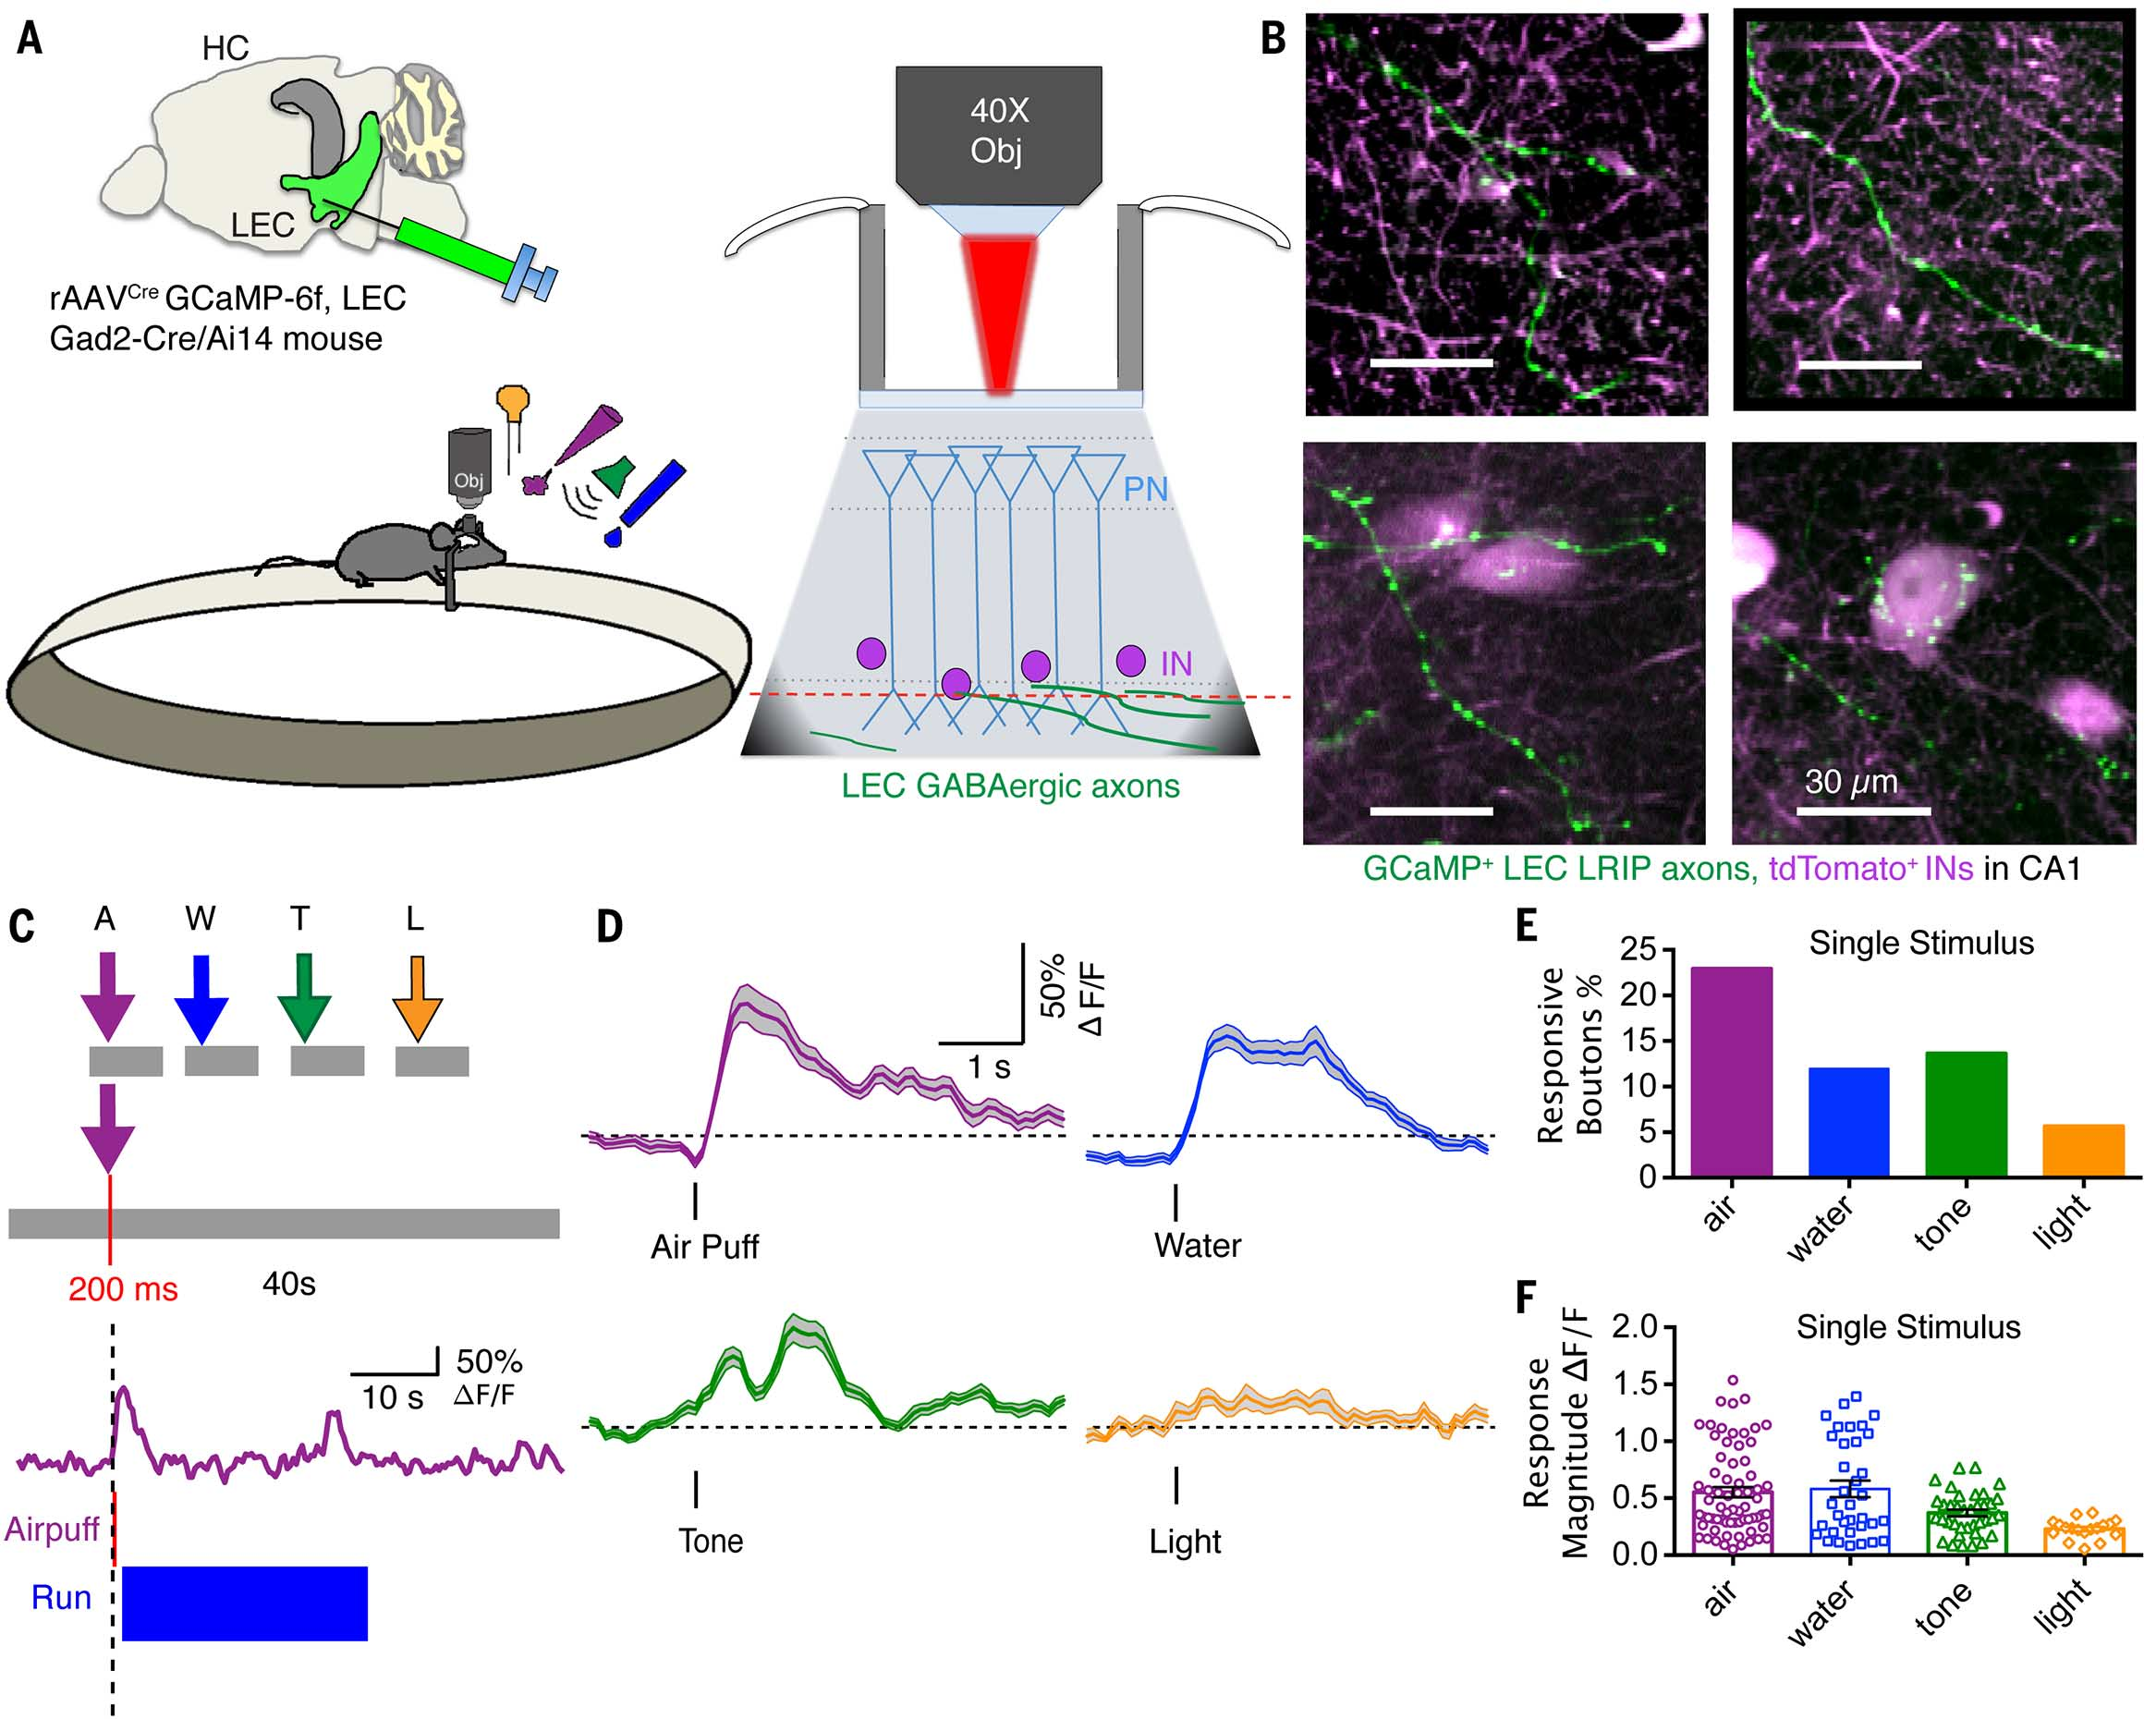
\includegraphics[width=0.75\textwidth]{applications/LRIP_Fig3_edit}
	\caption[Functional imaging of sensory coding in LEC LRIPs present in SLM of CA1]{Functional imaging of sensory coding in LEC LRIPs present in SLM of CA1.
	A) Diagram of in vivo imaging experiment. GCaMP6f was expressed in dorsal LEC, by injecting Cre-dependent rAAV in \emph{Gad2-Cre/Ai} 14 mice that also expressed tdTomato in all GABAergic neurons. A 40$\times$ water immersion objective was used for two-photon imaging through a cranial window over CA1 in head-fixed awake mice during multimodal sensory and behavioral stimuli presentation.
	(B) Four examples of time-averaged images of GCaMP6f fluorescence in LEC LRIP axons in SLM (green) with tdTomato labeling CA1 interneurons (magenta).
	(C) Experimental design of single-stimulus protocol. Imaging was performed in blocks of four trials, each 40 seconds in duration. After a 10~$\pm$~3~s baseline, one of four types of stimuli -- aversive air puff (A), water drop (W), tone (T), or light (L) -- was presented in random order for 200~ms, except the water drop was limited to 50~ms to prevent satiation. Each block was repeated to obtain at least five trials per stimulus. The animal's behavioral response (running and licking) was monitored. $\Delta F/F$ traces showing increased Ca\super{2+} signal in a single bouton on an LRIP axon in response to air puff.
	(D) Mean ($\pm$ SEM) $\Delta F/F$ Ca\super{2+} signal (PSTH) from responsive ROIs to indicated stimuli.
	(E) Percentage of responsive boutons to the stimuli (air~=~22.92\%, water~=~11.96\%, tone~=~13.64\%, and light~=~5.65\%).
	(F) Scatter and mean ($\pm$ SEM) plots of $\Delta F/F$ signals from individual responsive boutons (air~=~0.55~$\pm$~0.05, n~=~68; water~=~0.58~$\pm$~0.07, n~=~35; tone~=~0.37~$\pm$~0.03, n~=~37; light~=~0.23~$\pm$~0.02, n~=~18).
	% (G) Experimental protocol: Imaging was performed as described above, but in response to pairs of stimuli, presented in blocks of 10 trials, each 40 seconds long. Stimuli were randomized and paired stimuli were interleaved with single stimulus presentations.
	% (H) Mean ($\pm$ SEM) $\Delta F/F$ Ca\super{2+} signal (PSTH) from responsive ROIs to paired stimuli.
	% (I) Percentage of responsive boutons for paired stimuli (A+T~=~32.8\%; A+L~=~45.3\%; A+W~=~25.4\%; W+T~=~13.3\%; W+L~=~15.6\%; T+L~=~14.1\%).
	% (J) Scatter and mean ($\pm$ SEM) plots of $\Delta F/F$ signals to paired stimuli from individual responsive boutons (A+T~=~0.76~$\pm$~0.07, n~=~44; A+L~=~0.74~$\pm$~0.05, n~=~58; A+W~=~0.34~$\pm$~0.03, n~=~31; W+T~=~0.48~$\pm$~0.09, n~=~17; W+L~=~0.49~$\pm$~0.04; T+L~=~0.41~$\pm$~0.045, n~=~18).
	}
	\label{fig:applications:LRIP:imaging}
\end{figure}

\begin{figure}
	\centering
	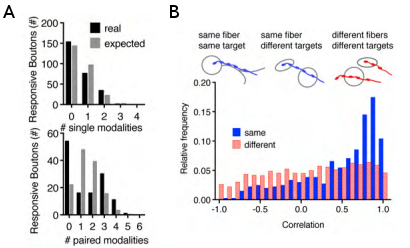
\includegraphics[width=0.75\textwidth]{applications/LRIP_FigS8_edit}
	\caption[Responsive properties of LRIP boutons]{Responsive properties of LRIP boutons. (A) Histogram bar plots of the number of responsive boutons (y axis) as a function of the number of stimulus modalities (x axis) to which a given bouton responds, either with a single sensory stimulus (above) or two stimuli presented simultaneously (below). The experimental data is plotted in black while the distribution expected if the stimuli and bouton responses were independent is in gray. For single stimulus presentations, very few boutons respond to more than one type of stimulus, following the predictions for independent responses (P~=~0.01659). In contrast, paired stimuli evoke Ca\super{2+} responses in a greater than expected number of boutons (P~$<$~0.03), perhaps the influence of a single overlapping stimulus in paired modalities (e.g. bouton responding to airpuff alone would likely respond to all three pairings with air; A+T, A+L, A+W).
	(B) Relative frequency distribution of bouton-bouton Ca\super{2+} response correlation coefficients for all identifiable bouton pairs originating from the same axon segment (solid blue, r~=~0.488 $\pm$ 0.017, n~=~808) versus boutons from different axons (cross-hatched red, r~=~0.115 $\pm$ 0.009, n~=~3992; P~$<$~0.0001, Mann-Whitney U test). Response similarity was determined by calculating the z-scored response magnitude for each stimulus for each bouton and then comparing the responses of pairs of boutons by calculating the correlation between their responses across all stimuli.
	}
	\label{fig:applications:LRIP:boutons}
\end{figure}


\section[Distinct Contribution of Adult-Born Hippocampal Granule Cells to Context Encoding]{Distinct Contribution of Adult-Born Hippocampal Granule Cells to Context Encoding\footnote{This work has been previously published \citep{Danielson2016a} and is joint work with the coauthors.}}

% In brief, dentate gyrus granule cells are one of the few populations of neurons that undergoes continue neurogenesis in the adult mammalian brain.
\begin{quote}
Adult-born granule cells (abGCs) have been implicated in cognition and mood; however, it remains unknown how these cells behave in vivo. Here, we have used two-photon calcium imaging to monitor the activity of young abGCs in awake behaving mice. We find that young adult-born neurons fire at a higher rate in vivo but paradoxically exhibit less spatial tuning than their mature counterparts. When presented with different contexts, mature granule cells underwent robust remapping of their spatial representations, and the few spatially tuned adult-born cells remapped to a similar degree. We next used optogenetic silencing to confirm the direct involvement of abGCs in context encoding and discrimination, consistent with their proposed role in pattern separation. These results provide the first in vivo characterization of abGCs and reveal their participation in the encoding of novel information.
\attrib{\citealt{Danielson2016a}}
\end{quote}

While this project is the primary work of the first author, the behavioral apparatus, experimental paradigms, and analysis tools were all developed jointly.
In particular, this manuscript was Attila Losonczy's lab's first publication of head-fixed two-photon calcium imaging of place cells in mice, so relied upon upgrades to the behavioral apparatus (\autoref{sec:intro:techniques:behavior}), the imaging processing pipeline (\autoref{sec:intro:techniques:pipeline}), and analysis of place cell data (\autoref{sec:intro:techniques:place-cells}).

\begin{figure}
	\centering
	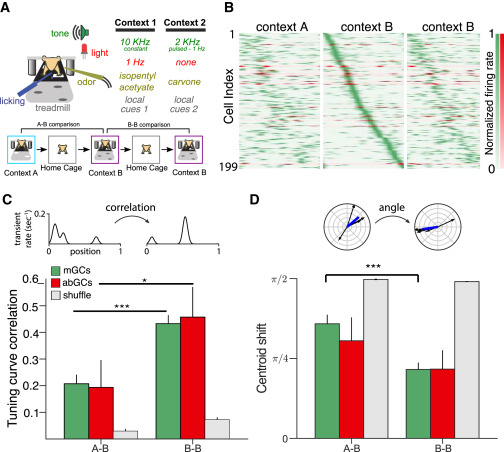
\includegraphics[width=0.8\textwidth]{applications/abGC_Fig3}
	\caption[Contextual coding by adult-born and mature granule cells]{Contextual coding by adult-born and mature granule cells.
	A) Experimental schematic. Mice ran for three 12-min sessions in contexts A, B, and B (1 hr between runs). A and B refer to either context 1 or 2 (chosen randomly for each experiment).
	(B) Remapping of spatial rate maps across sequential context exposures. Smoothed calcium transient rates, normalized to peak for each cell, are plotted as a function of position during three contextual exposures (A, B, B). Cells (mGCs, green; abGCs, red) are ordered according to the position of peak activity during the first exposure to context B. Data is shown for GCs with sufficient tuning specificity and activity (p~$<$~0.1, at least four transients) in at least one experiment.
	(C and D) Context specificity of spatial representations. Tuning curve correlations of 1D rate maps (C) and centroid shifts (angle between tuning directions) (D) between sequential exposures to different (A-B) or the same (B-B) contexts for all cells shown in (B) (A-B: n~=~180 mGCs, 14~abGCs; B-B: n~=~174 mGCs, 9~abGCs). The rate map correlations of both populations were more similar in the B-B condition than in A-B (Mann-Whitney U, mGCs: U(150)~=~5,291, p~$<$~0.001; abGCs: U(18)~=~23.0, p~$<$~0.05). In mGCs the tuning shift was larger in the A-B condition than in B-B, although this did not reach significance in abGCs (mGCs: U(150)~=~5,714, p~$<$~0.001; abGCs: U(18)~=~40.0, p~=~0.34). In both conditions, the similarity of spatial representations exceeded chance levels as estimated by shuffling cell identity (gray).
	Error bars are mean~$\pm$~SEM.}
	\label{fig:applications:dg:context}
\end{figure}

\section[Sublayer-Specific Coding Dynamics during Spatial Navigation and Learning in Hippocampal Area CA1]{Sublayer-Specific Coding Dynamics during Spatial Navigation and Learning in Hippocampal Area CA1\footnote{This work has been previously published \citep{Danielson2016b} and is joint work with the coauthors.}}

\begin{quote}
The mammalian hippocampus is critical for spatial information processing and episodic memory. Its primary output cells, CA1 pyramidal cells (CA1 PCs), vary in genetics, morphology, connectivity, and electrophysiological properties. It is therefore possible that distinct CA1 PC subpopulations encode different features of the environment and differentially contribute to learning. To test this hypothesis, we optically monitored activity in deep and superficial CA1 PCs segregated along the radial axis of the mouse hippocampus and assessed the relationship between sublayer dynamics and learning. Superficial placemaps were more stable than deep during headfixed exploration. Deep maps, however, were preferentially stabilized during goal-oriented learning, and representation of the reward zone by deep cells predicted task performance. These findings demonstrate that superficial CA1 PCs provide a more stable map of an environment, while their counterparts in the deep sublayer provide a more flexible representation that is shaped by learning about salient features in the environment.
\attrib{\citealt{Danielson2016b}}
\end{quote}

This project was the primary work of the first author, Nathan Danielson, but again a lot of the experimental designs, tools, and procedures were developed collaboratively: \ac{GOL} task (\autoref{sec:intro:techniques:GOL}, \autoref{fig:applications:sf-deep:GOL}), place cell stability metrics (\autoref{sec:intro:techniques:place-cells}, \autoref{fig:applications:sf-deep:stability}), and reward enrichment analysis (\autoref{fig:applications:sf-deep:enrichment}).

\begin{figure}
	\centering
	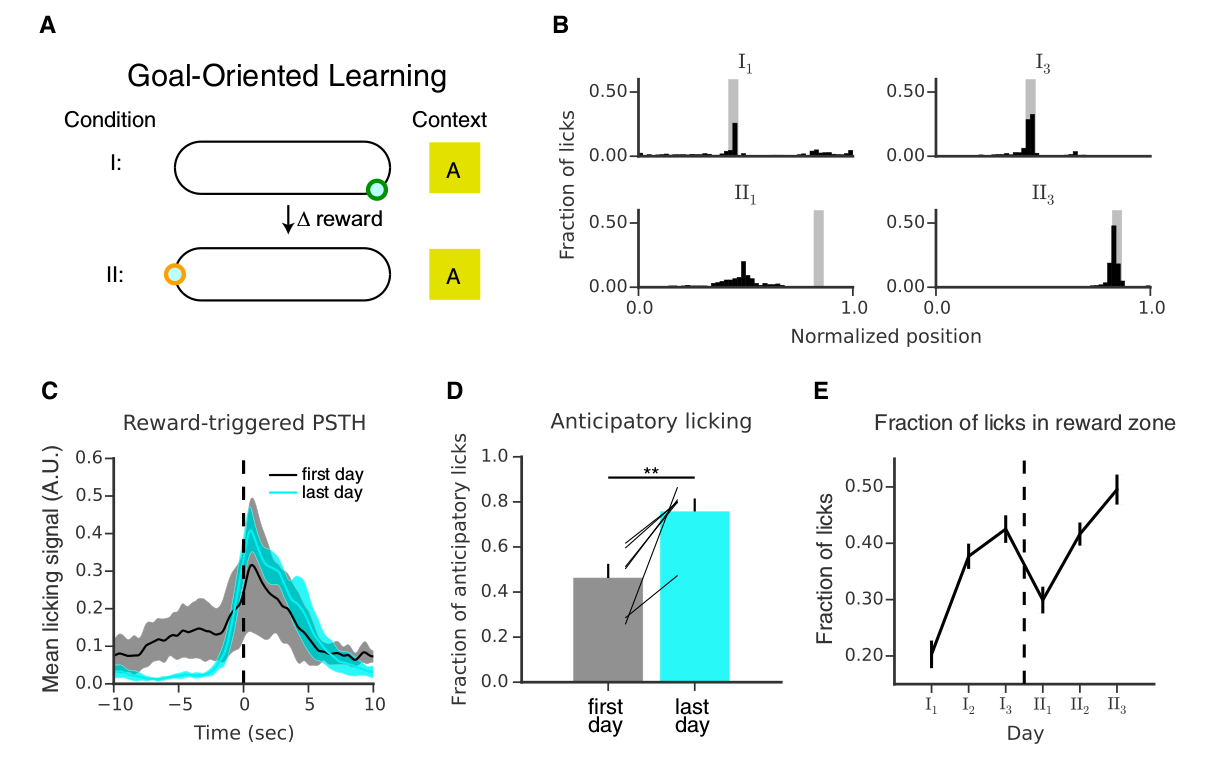
\includegraphics[width=0.8\textwidth]{applications/sf_deep_Fig3}
	\caption[GOL Task for Head-Fixed Imaging]{GOL Task for Head-Fixed Imaging.
	(A) Schematic of the goal-oriented learning (GOL) task. Mice (n~=~6) searched for an unmarked reward zone, and water rewards were administered only when the mice licked within the fixed 10-cm goal. At the end of condition I, the reward was moved to a new location of the belt, and the experiment was repeated (condition II). The same context (A) was maintained throughout.
	(B) Representative licking data from four individual experiments from one mouse performing the task. The fraction of total licks is plotted as a function of position on the belt (50 bins, 4 cm per bin). The reward zone is shaded gray. On the first day of the experiment, the mouse licked diffusely throughout the belt as it searched for the hidden reward zone. By the last day of condition I, the mouse licked selectively at the reward location. After the reward was moved, the mouse continued to lick at the original reward location. It eventually reverted to an exploratory licking state, and by the end of condition II the mouse selectively licked at the new reward location.
	(C) Peri-stimulus time histogram (PSTH) of licking rate triggered on reward zone entry for the first (black) and last (cyan) days of each condition. PSTHs were calculated for each mouse and smoothed with a 1-s Hamming filter. Shaded regions indicate mean $\pm$ SD across mice. Licking was initially diffuse. By the last day, licking outside the reward zone was largely suppressed and rose sharply prior to reward zone entry, reflecting the expectation of reward. The effect was highly consistent across mice.
	(D) Anticipatory licking (fraction of non-reward zone licks in the 10~cm preceding the reward) increased significantly by the end of learning (n~=~6 mice, p~$<$~0.01, paired t-test). Error bars indicate mean $\pm$ SEM across mice.
	(E) The fraction of licks occurring within the reward zone aggregated by recording session and plotted by day (mean $\pm$ SEM across mice). Over time, licking became more selective for the reward zone.
	}
	\label{fig:applications:sf-deep:GOL}
\end{figure}

\begin{figure}
	\centering
	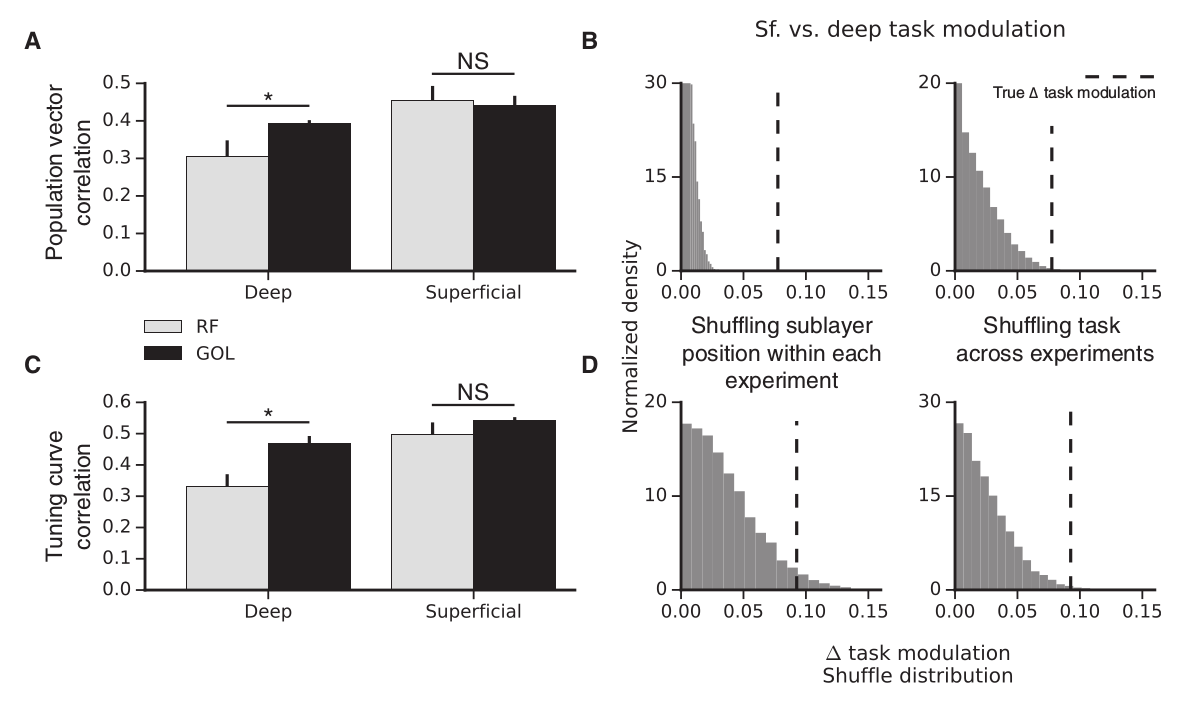
\includegraphics[width=0.8\textwidth]{applications/sf_deep_Fig4}
	\caption[Sublayer-Specific Modulation of Activity by the GOL Task]{Sublayer-Specific Modulation of Activity by the GOL Task.
	(A) Stability in the B-B condition of RF compared to session-to-session stability in GOL (similar elapsed time of $~$90~min.). Deep, but not superficial, CA1 PCs showed a significant increase in PV correlation in the GOL task as compared to RF (n~=~7 RF mice, 6 GOL mice; deep, p~$<$~0.05; superficial, p~=~0.36; Mann-Whitney U test). Error bars indicate mean $\pm$ SEM across animals.
	(B) The magnitude of the task modulation was compared across sublayers by performing two shuffling procedures: randomizing cell identity and randomizing task identity. Both comparisons suggested the magnitude of task modulation was greater for deep than for superficial cells (p~$<$~0.001, p~$<$~0.01).
	(C) The same analysis was performed with tuning curve correlation. Deep, but not superficial, CA1 PCs showed a significant increase in tuning curve correlation in the GOL task as compared to RF (n~=~7 RF mice, 6 GOL mice; deep, p~$<$~0.05; superficial, p~=~0.11; Mann-Whitney U test). Error bars indicate mean $\pm$ SEM across animals.
	(D) Both shuffles showed the magnitude of the task modulation was greater for deep than superficial (p~$<$~0.01, p~$<$~0.01).
	}
	\label{fig:applications:sf-deep:stability}
\end{figure}

\begin{figure}
	\centering
	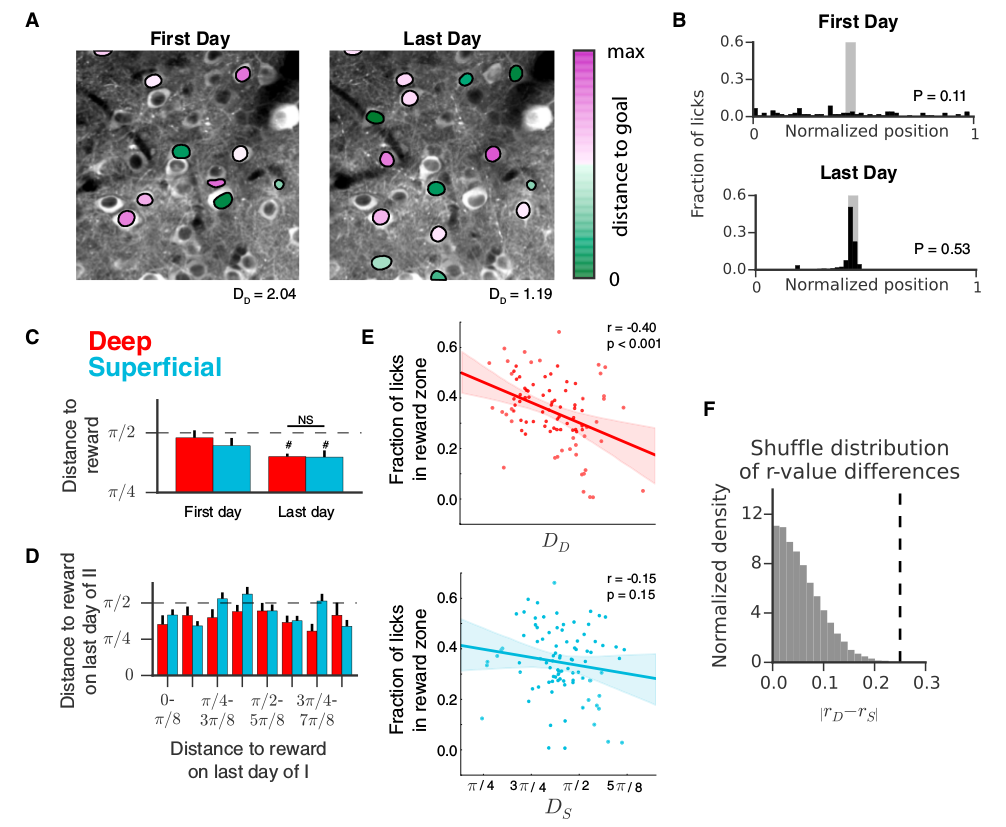
\includegraphics[width=0.8\textwidth]{applications/sf_deep_Fig6}
	\caption[Reward Zone Representation versus Performance on the GOL Task]{Reward Zone Representation versus Performance on the GOL Task.
	(A) Time-averaged images of the deep sublayer from two different recording sessions are shown in grayscale. Identified place cells from each session are overlaid and colored according to the distance of their centroid to the reward (green, near; purple, away). The mean distance to the reward zone is indicated (radians).
	(B) As in \autoref{fig:applications:sf-deep:GOL}B, licking distributions from the two experiments corresponding to (A).
	(C) Mean distance of each place cell centroid to the reward on first and last days of the experiment. On the last day, the mean distance to reward was significantly different from the chance level of $\pi$/2 for both sublayers (dashed line; n~=~6 mice; one sample t-test; deep, p~$<$~0.001; superficial, p~$<$~0.05), but was not significantly different between sublayers (n~=~6 mice, p~=~0.95, paired t-test). Error bars indicate mean $\pm$ SEM across animals.
	(D) We did not detect a relationship between distance to reward at the end of condition II with distance at the end of I, sublayer, or with the interaction (type II ANOVA, n~=~172 deep, 336 superficial place cells, F(distance end of I)~=~0.10, p(distance end of I)~=~0.76; F(layer)~=~0.54, p(layer)~=~0.46; F(interaction)~=~0.11, p~=~0.74). The dashed line represents the mean distance expected in the case of a uniform place field distribution, and error bars indicate mean $\pm$ SEM across cells.
	(E) Fraction of licks in reward zone (P) plotted against D\sub{D} (top) and D\sub{S} (bottom). Individual points represent single recording sessions. The dashed line indicates the linear fit with the 95\% confidence interval shaded. We observed a significant relationship between D\sub{D} and P (n~=~91 sessions, r~=~0.40, p~$<$~0.001, Pearson's R), but not between D\sub{S} and P (n~=~91 sessions, r~=~0.15, p~=~0.15, Pearson's R).
	(F) In order to directly compare the sublayers' relationships to performance on the GOL task, we compared the magnitude of the difference in correlation coefficients (0.25, dashed line) relative to a null distribution. The true difference (dashed line) fell outside the shuffle distribution (p~$<$~0.001).
	}
	\label{fig:applications:sf-deep:enrichment}
\end{figure}
\todo[inline]{Expand on sf-deep results}